\begin{gbox}{}{grey1}{\hspace*{4cm}{\large \textbf{Multi-Unit Spectroscopy
        Explorer (MUSE)}}}
  \begin{minipage}{\linewidth}
    \begin{wrapfigure}{r}{0pt}
      \includegraphics[width=15cm]{MUSE/MUSE.png}
    \end{wrapfigure}
    \strut {\small MUSE is a second
      generation instrument in development for the Very Large Telescope (VLT) of
      the European Southern Observatory (ESO). MUSE couples the
      discovery potential of an imaging device to the measuring capabilities of
      a spectrograph, while taking advantage of the increased spatial resolution
      provided by adaptive optics. This makes it a unique and powerful tool for
      discovering objects that cannot be found in imaging surveys.}
  \end{minipage}

  \begin{minipage}{\linewidth}
    \begin{wrapfigure}{l}{0pt}
      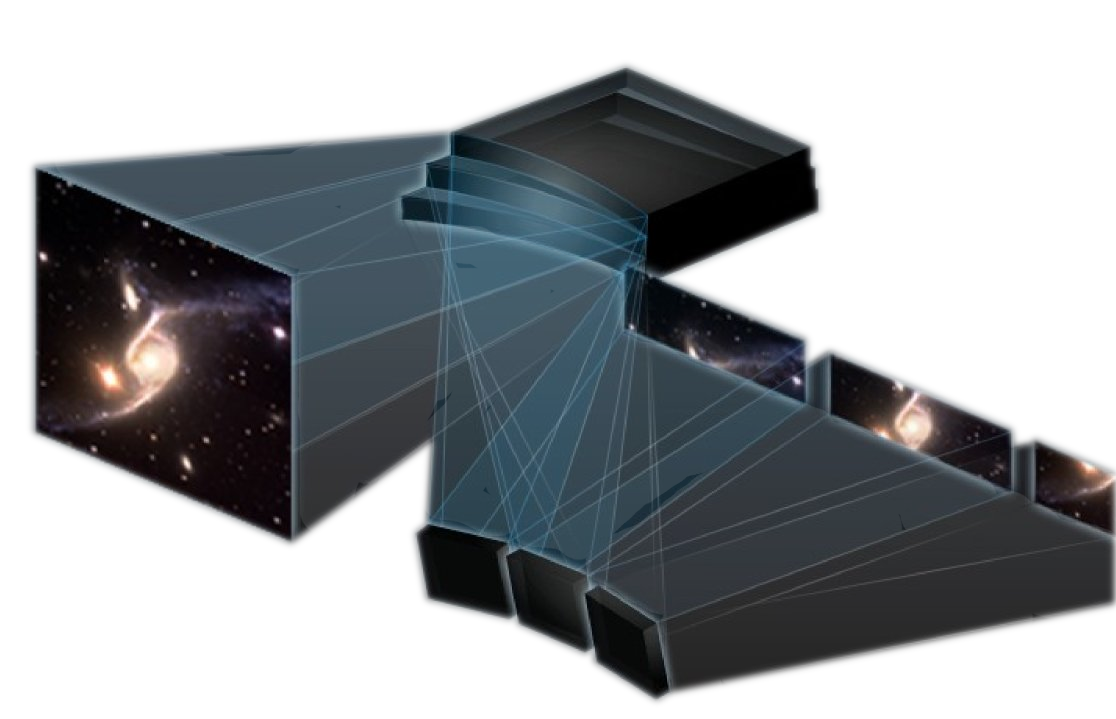
\includegraphics[width=10cm]{MUSE/MUSE_slicer_schematic.png}
    \end{wrapfigure}
    \strut {\small The concept of MUSE foresees the splitting of the adaptive
      optics corrected field of view in 24 sub-fields. Each of these sub-fields
      is fed into a spectrograph (called Integral Field Unit, IFU). An image
      slicer in front of each IFU serves as entrance slit, thus producing a
      spatially resolved spectrum of the full sub-field (from ESO
      website).}
  \end{minipage}

  \vspace{2cm}

  \begin{minipage}{\linewidth}
    \begin{center}
      
\includegraphics[height=3cm]{MUSE/logos.png}
    \end{center}
  \end{minipage}
\end{gbox}